\documentclass[a4paper]{jpconf}
\usepackage{graphicx}
\usepackage{amsmath}
\usepackage{bm}
\begin{document}
\title{Design of a bend-twist coupled blade for a small wind turbine using multidisciplinary optimisation}

\author{Antariksh Dicholkar$^1$, Frederik Zahle$^1$, Michael McWilliam$^1$, Taeseong Kim$^1$ and Jessica Holierhoek$^2$}

\address{$^1$ DTU Wind Energy, DTU Ris{\o} campus, Frederiksborgvej 399, DK-4000 Roskilde}
\address{$^2$ Faculty of Aerospace Engineering, TU Delft, Kluyverweg 1, 2629 HS Delft, The Netherlands}

\ead{acdi@dtu.dk}
%%---------------------------------------------------------------------------------------------------------------------------
%%--------------------------------------------------------------------------------------------------------------------------
\begin{abstract}
The present study focuses on including bend-twist coupling (BTC) in the design of a 500W rotor by using a combination of parametric studies and a Multidisciplinary Design Optimisation (MDO) approach. The effectiveness of BTC is gauged through obtaining a significant decrease in the flapwise blade root bending moment with a marginal decrease in the AEP. Carbon outperforms glass for all fibre angles with regard to the amount of coupling observed. Apart from flapwise bend-twist coupling, other secondary torsion couplings are also present that alter the desired BTC. The steady state load response of the blade is assessed for varying positive fibre layup angles. The reduction in the flapwise bending loads is not significant due to insufficient degree of induced torsion. These factors justify an MDO approach. The HawtOpt2 aero-structural design tool is utilised to implement the MDO of the baseline blade. The spanwise fibre layup angle and laminate thickness distribution are the only structural design variables being varied along with planform, blade length and rotor speed. The objective function seeks to minimise extreme flapwise bending loads and maximise the AEP through a multi-objective optimisation, with the individual objectives being linearly scaled by complementary weights.
\end{abstract}
%%--------------------------------------------------------------------------------------------------------------------------
%%-------------------------------------------------------------------------------------------------------------------------
\section{Introduction}
\label{sec:intro}
Passive control of wind turbine rotors through the mechanism of material Bend-Twist Coupling (BTC) has been extensively addressed in existing literature \cite{veers1998aeroelastic}. %\cite{kooijman1996bending}, \cite{karaolis1988active}. 
While early research focused on achieving power regulation by BTC towards stall on stall-regulated constant speed rotors 
%\cite{lobitz1996enhanced}, \cite{lobitz1999load} 
, the advent of pitch regulated variable speed control strategy pivoted the research towards utilising BTC towards feather for passive load alleviation. %\cite{lobitz2003load}, \cite{lobitz2000performance}, \cite{capellaro2012design}. 
However, most of the research is focused on the usage of BTC for multi-megawatt turbines with little research being conducted on small wind turbines. The present study focuses on including BTC towards feather as a mechanism for passive load alleviation, in the design of a 500W rotor by using a combination of parametric studies and a Multidisciplinary Design Optimisation (MDO) approach. The effectiveness of BTC is assessed by a decrease in the flapwise blade root bending moment with a marginal decrease in the Annual Energy Production (AEP), compared with a baseline turbine.

%The challenge lies in developing an approach which incorporates BTC in the rotor, satisfying the multiple design constraints and presents feasible alternatives. These alternatives then have to be qualified according to their performance with only the best being carefully selected, thus resulting in a optimally performing turbine. This can be a complicated task due to the inter-dependencies of the different design requirements. The presence of complex relationships between design variables and the significant number of such variables necessitates numerical optimisation to carry out multidisciplinary design.% \cite{bottasso2012multi}, \cite{zahle2016design}.
Design investigations into BTC are complicated by the multiple design constraints. Incorporating BTC in an otherwise unmodified blade will likely result in constraints being violated, which in-turn require other design variables to be modified to make the rotor feasible again. Thus, to fully understand the impact of BTC, the whole design space needs to be considered simultaneous. To overcome this challenge design optimisation is required.

This study is an extension to the work conducted in the master thesis of Dicholkar \cite{dicholkar2017numerical}, wherein only a structural optimisation was performed. The structural design variables of spanwise fibre layup angle and laminate thickness distribution were varied in the design. The objective here was on minimising extreme flapwise bending loads. In the present paper, the HawtOpt2 \cite{zahle2016design} aero-structural design tool is utilised to perform the MDO of the baseline blade and a second blade with BTC for comparison. This paper will build on the work already done, by considering additional design variables like planform, blade length and rotor speed. A multi-objective optimisation will be carried out to identify the optimal trade-off between AEP and the extreme flapwise bending loads, by linearly scaling the objectives with complementary weights. 
%The HawtOpt2 \cite{zahle2016design} aero-structural design tool is utilised to perform the MDO of the baseline blade and a second blade with BTC for comparison. This study is an extension to the work conducted in the master thesis of Dicholkar \cite{dicholkar2017numerical}, wherein only the structural design variables of spanwise fibre layup angle and laminate thickness distribution were varied in the design. The objective here was on minimising extreme flapwise bending loads. This paper will build on this work by considering additional design variables like planform, blade length and rotor speed. A multi-objective optimisation will be carried out to identify the optimal trade-off between AEP and the extreme flapwise bending loads, by linearly scaling the objectives with complementary weights.
%Additionally, the objective function seeks to minimise extreme flapwise bending loads and maximise the AEP through a weighted function. The performance of the optimised blades are to be compared for multiple combinations of the assigned weights. 


%The previous optimisation studies performed with Hawtopt2 have focused on multi-megawatt turbines, namely the DTU 10 MW reference turbine \cite{DTU10MW_1}. Zahle et. al \cite{zahle2016design} performed an aero-structural optimisation of the DTU 10MW reference rotor to maximise the annual energy production (AEP) without exceeding the design loads of the reference. Pavese et. al \cite{pavese2017design}, \cite{pavese2017aeroelastic} optimized the pre-twist distribution of swept blades designed based on the DTU 10 MW rotor. Barlas et al. \cite{barlas2016aeroelastic} conducted an aero-structural optimization of the DTU 10 MW rotor with active trailing edge flaps by assigning design freedom to the blade planform and material layup. In another study, Pavese et al. \cite{pavese2016reduced} formulated a reduced design load basis (DLB) approach that captured the effect of turbulent inflow by utilising simulated shear and extreme operating gusts, and was applied in the aero-structural optimisation of the DTU 10 MW rotor. Wandji et al. \cite{wandji2016reduction} performed an aero-structural optimisation of the DTU 10 MW rotor to minimise tower bottom fatigue loads without significant loss in AEP by utilising a weighted composite objective function.  

%This paper seeks to utilise the HawtOpt2 tool to perform an aero-structural optimisation of a 500W rotor and introduce bend-twist coupling in the process. The baseline blade being optimised for passive load alleviation is fundamentally different to that of the DTU 10 MW and operates in a different wind climate. With a much greater normalised solidity and stiffness along with smaller design loads, the limitations of the prescribed MDO workflow will inadvertently be tested.   

\section{Method}
\label{sec:method}
To properly evaluate material BTC, the cross section analysis tool BECAS \cite{becas1} is used to calculate the full 6x6 stiffness matrix. BECAS is a finite element based tool that takes into account the full anisotropy of the materials. 

The baseline blade is designed using a conventional sequential design approach and has a length of 0.79 m with a uniform laminate thickness of 1 mm. Three parametric studies are conducted on the baseline blade by discretely varying the fibre orientations for the last 60\% of the span.

The first parametric study focuses on analysing the bend-twist properties and the cross-sectional stiffnesses for both glass and carbon fibre blades.

The next parametric study examines the steady-state performance of the bend-twist coupled blades by using the aeroelastic tool HAWC2 \cite{hawc2}. The bending moments, airfoil performance and power production are evaluated.

The final parametric study looks at the impact of BTC towards feather on the damage equivalent loads.

The baseline wind turbine blade is aero-structurally optimised using HawtOpt2. The maximum allowable blade tip deflection is constrained and the loads are limited to the design loads of the uncoupled blade. The multi-objective function to be minimised is shown in Equation \ref{eq:objective_function}.
\begin{equation}
\resizebox{.9 \textwidth}{!}{ 
     $ f(\{\bm{x_p}, \bm{x_s}, \bm{x_{oper}}\},\bm{p}, w)= -\left( w \cdot \dfrac{AEP(\{\bm{x_p}, \bm{x_s}, \bm{x_{oper}}\},\bm{p})}{AEP(\{\bm{0},\bm{0},\bm{0}\},\bm{p})} + (1-w) \cdot \dfrac{M_x(\{\bm{0},\bm{0},\bm{0}\},\bm{p})}{M_x(\{\bm{x_p}, \bm{x_s}, \bm{x_{oper}}\},\bm{p})} \right)$
     }
\label{eq:objective_function}
\end{equation}
where $f$ represents the cost function, $AEP$ is the annual energy production, $M_x$ is the extreme flapwise blade root bending moment, $w$ is the weight given to the aerodynamic and structural parameters that determines the trade-off, $x_p$ are the collection of the blade planform design variables, $x_s$ is the collection of the blade structural variables, $x_{oper}$ is the collection of wind turbine control variables and $p$ represents the variables that are kept constant. $AEP(\{0,0,0\},p)$ and $M_x(\{0,0,0\},p)$ represent the AEP and the flapwise root bending moment for the baseline uncoupled rotor, respectively.

\section{Preliminary results and conclusions}
\label{sec:results}
The flapwise BTC with twisting towards feather occurs for positive fibre layup angles on the pressure side of the blade sections. This is facilitated by negative values of the torsion coupling terms. Figures \ref{subfig:carbonVglass_flapvedgetors_40} and \ref{subfig:carbonVglass_otherstifftors_40} indicate the presence of secondary torsion couplings along with the primary flapwise BTC. These secondary couplings would contribute to the final value of the induced torsion and thus either positively or negatively affect the desired outcome of BTC. Furthermore, the contributions of the secondary couplings cannot be precisely quantified.      
%----------------Comparision of stiffnesses-----------
\begin{figure}[pth]
\centering
\begin{minipage}{0.45\textwidth}
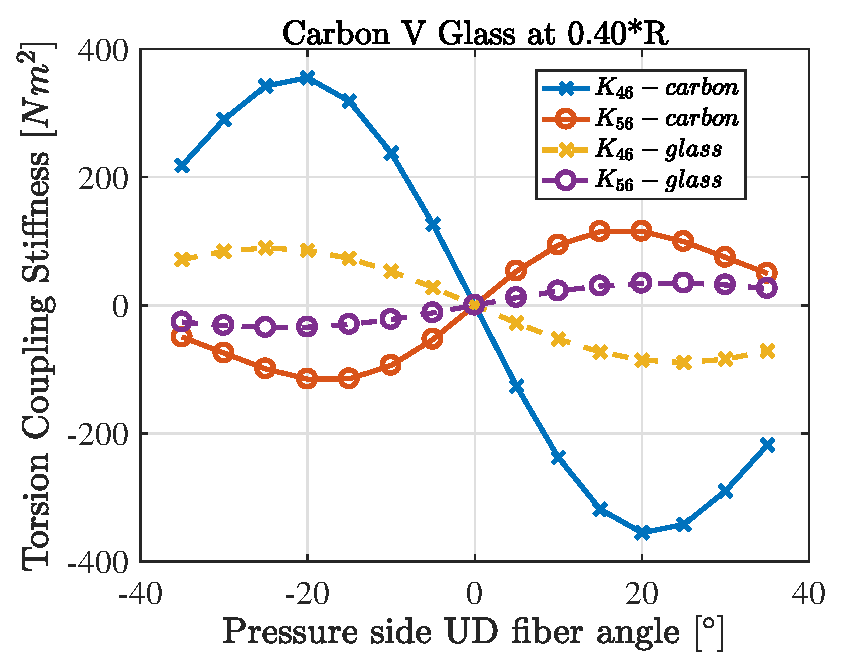
\includegraphics[width=\linewidth]{Figures/Chapter4/Stiffness/CarbonVglass_flapVedgecoupl_40_eps.eps}
\caption{\label{subfig:carbonVglass_flapvedgetors_40}Flap-torsion $K_{46}$ and edge-torsion $K_{56}$ coupling stiffness terms at 40\% blade span.}
\end{minipage}\hspace{0.10\textwidth}%
\begin{minipage}{0.45\textwidth}
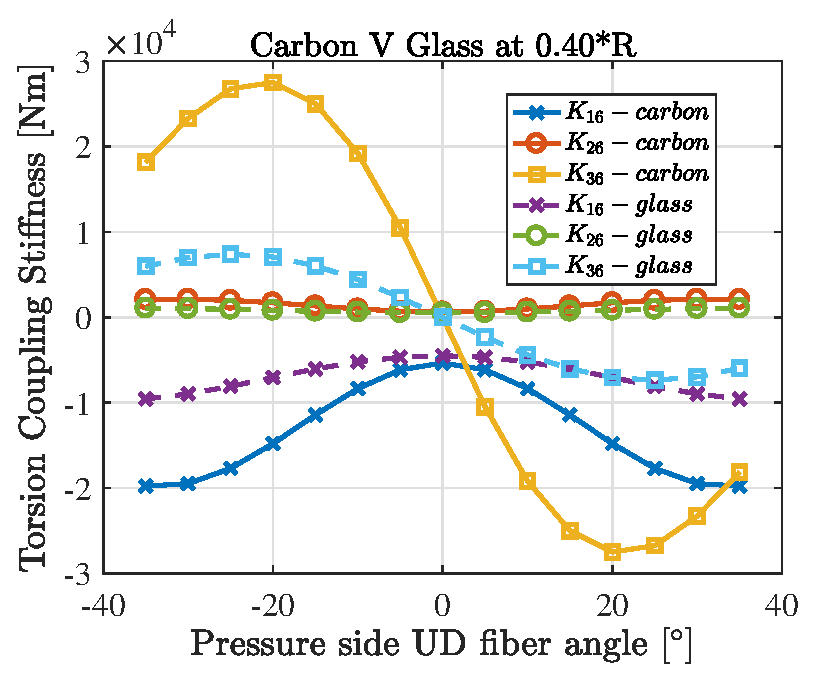
\includegraphics[width=\linewidth]{Figures/Chapter4/Stiffness/CarbonVglass_otherstiffcoupl_40_eps.eps}
\caption{\label{subfig:carbonVglass_otherstifftors_40}Edgewise shear-torsion $K_{16}$, flapwise shear-torsion $K_{26}$ and axial-torsion $K_{36}$ coupling stiffness terms at 40\% blade span.}
\end{minipage} 
\end{figure}
%----------------------------------

Figure \ref{subfig:mx_rel} shows the greatest relative decrease in the flapwise blade root bending moment to be 2.8\% at a pressure side fibre layup angle of 25$^\circ$ in the carbon fibre blade. The small reduction in the extreme flapwise bending load is due to the decrease in angle of attack not being significant enough for the airfoil to operate at a sub-optimal lift to drag ratio. This is due to the induced torsion towards feather not being sufficiently large. Since only one airfoil series is used throughout the blade, this reasoning holds for the power producing mid and near tip region of the span. The relative change in the airfoil angle of attack near the tip is shown in Figure \ref{subfig:alphacurve_rel}.


%----------------Comparision of load response-----------
\begin{figure}[pth]
\centering
\begin{minipage}{0.45\textwidth}
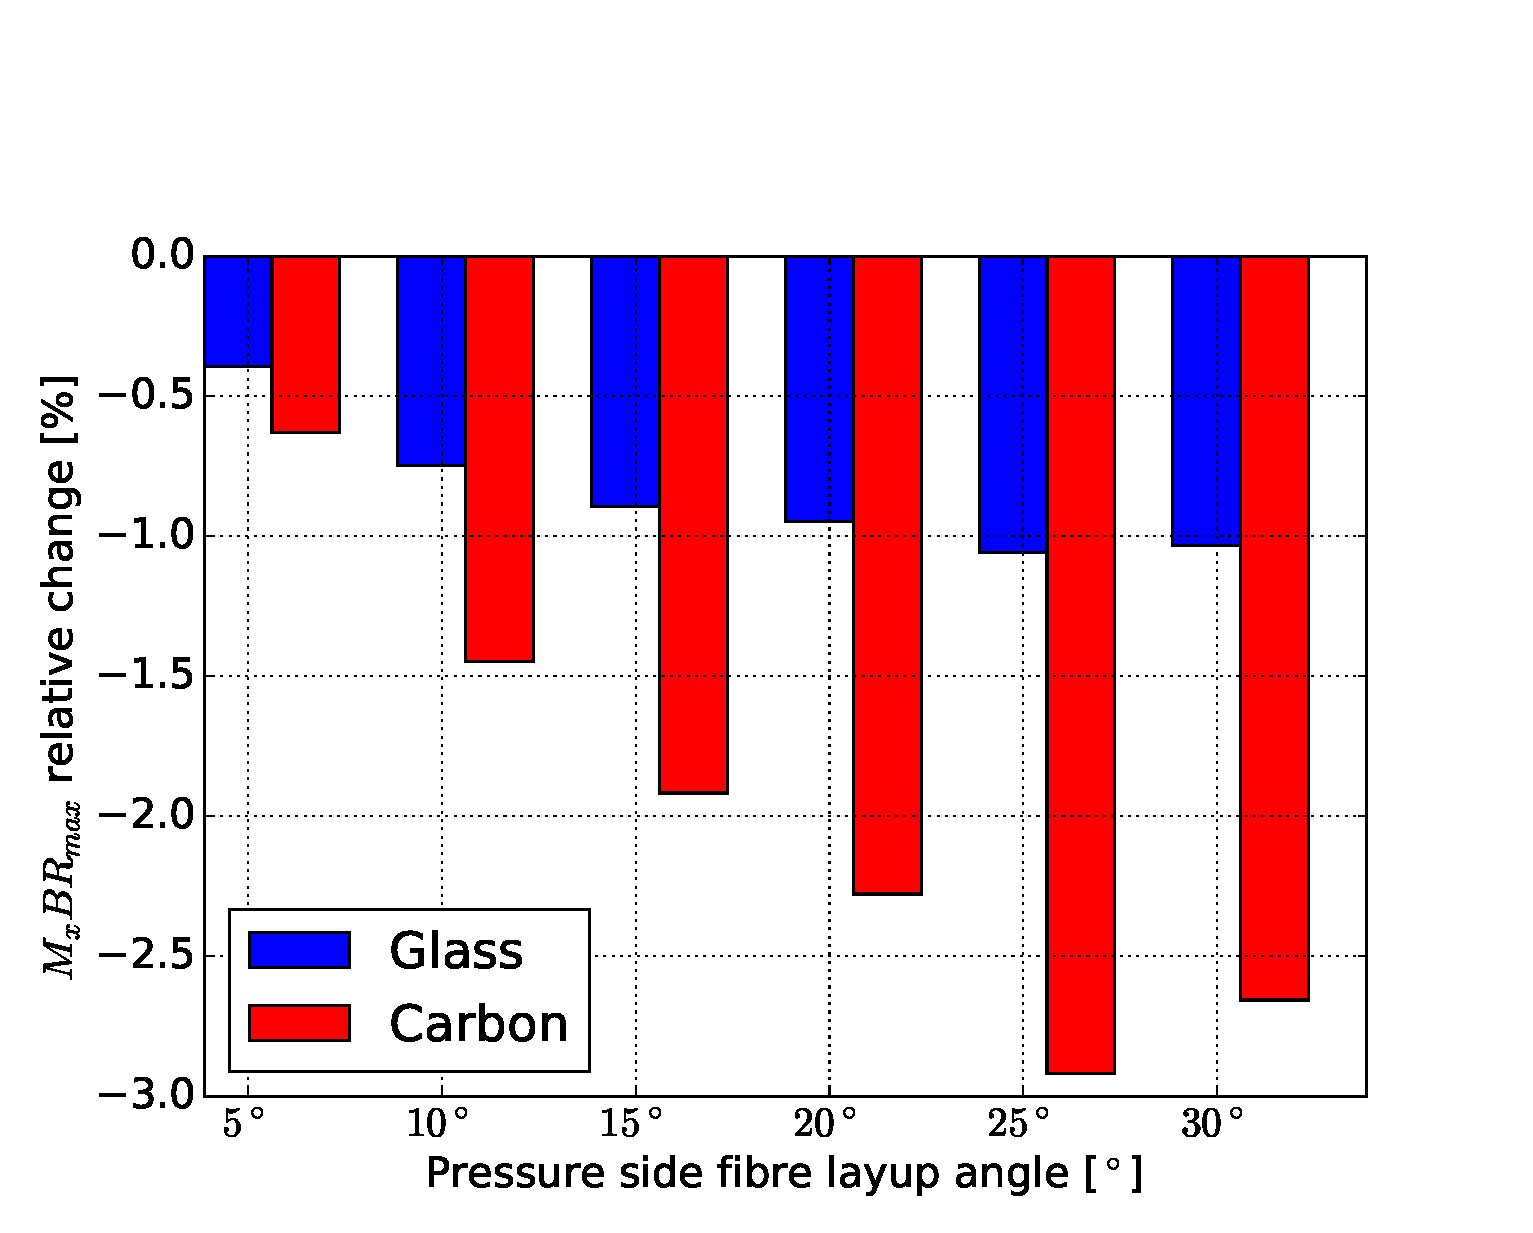
\includegraphics[width=\linewidth]{Figures/Chapter4/Load/steady_relmxbr.eps}
\caption{\label{subfig:mx_rel}Change in maximum flapwise root bending moment $M_xBR_{max}$ relative to the uncoupled blade for 10m/s rated wind speed.}
\end{minipage}\hspace{0.10\textwidth}%
\begin{minipage}{0.45\textwidth}
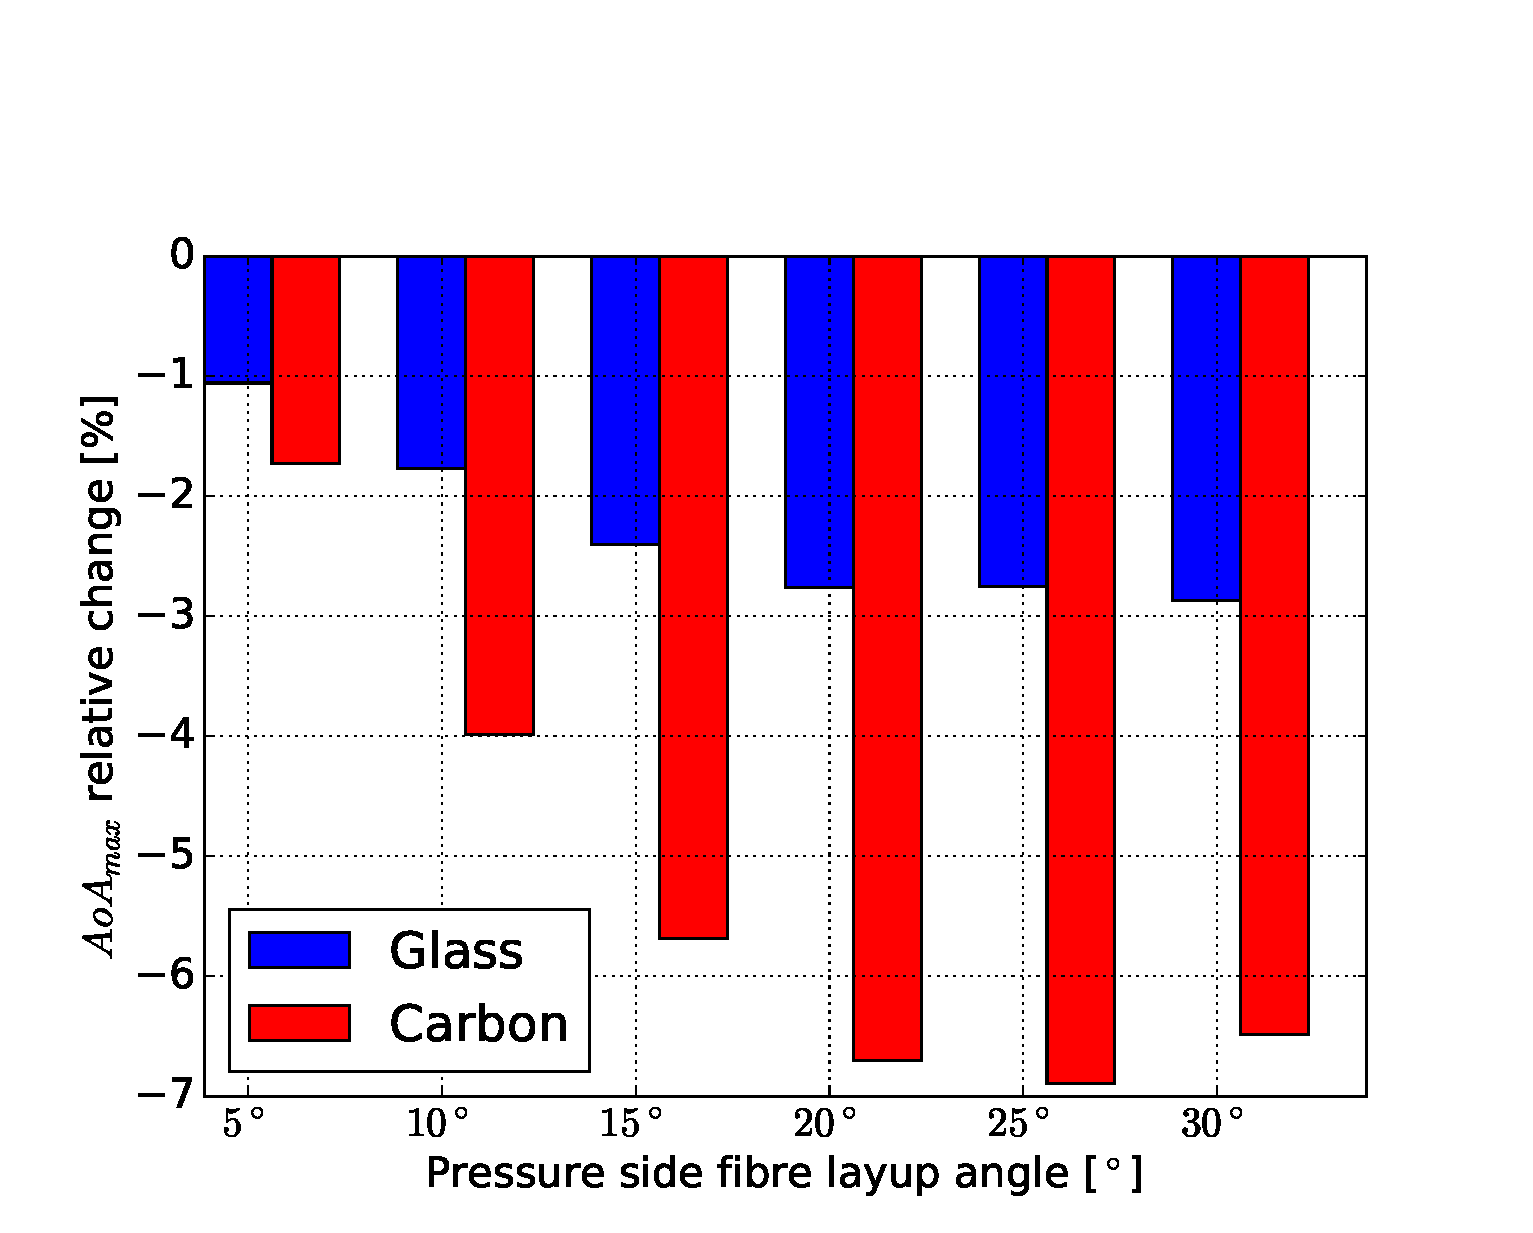
\includegraphics[width=\linewidth]{Figures/Chapter4/Load/steady_relalpha.eps}
\caption{\label{subfig:alphacurve_rel}Change in $AoA_{max}$ relative to the uncoupled case for 10m/s wind speed, at 87\% blade span.}
\end{minipage} 
\end{figure}
%----------------------------------

%\section{Preliminary conclusion}
%\label{sec:conclusion}
 Carbon outperforms glass for all positive pressure side fibre angles with regard to the amount of coupling seen in the blade cross-sections. Apart from flapwise bend-twist coupling, other secondary torsion couplings are also present. The small amount of reduction in the flapwise blade root bending moment points to a low degree of induced torsion as a result of the high prevalent torsional stiffness in the baseline blade. Since the blade already has a laminate thickness at the minimum manufacturing limit, a further reduction cannot be justified. Hence, a purely structural optimisation through changes in the spanwise laminate fibre layup angles may not be sufficient to produce an effective BTC blade. However, a reduction in the cross-sectional stiffnesses can positively influence this outcome to a large extent. The cross-sectional stiffnesses scale with the cube of the local chord and thus, altering the planform could lead to an improved BTC response. But this will also have an effect on the power production. This could in turn be remedied by an increase in the rotor area, which would consequently increase the bending loads. Such complexities in the design justify the need for an aero-structural MDO.    

%% Add the bibliography according to style iopart-num.bst
\section*{References}
\bibliographystyle{iopart-num.bst}
\bibliography{references.bib}

\end{document}


